\chapter{Capturing a Light Field}
\label{chp:light_field_capturing}

\todo{Add small introduction}

\section{The Plenoptic Function and the Light Field}

The plenoptic function, as introduced by~\cite{AdelsonBergen}, is a 7D function that describes the intensity of light for every frequency, along every light ray in space, at any time. 
It is defined as
\begin{align*}
	P \colon \mathbb{R}^3 \times \left[0, 2 \pi \right) \times \left[ 0, \pi \right] \times \mathbb{R}^2 & \to \mathbb{R}^+ \\
	\left(x, y, z, \theta, \phi, t, \lambda \right) & \mapsto P\left(x, y, z, \theta, \phi, t, \lambda \right), 
\end{align*}
where the parameters $\left(x, y, z\right)$ are the coordinates of a point in 3D space and the angles $\left(\theta, \phi \right)$ describe the direction of an incoming light ray at time $t$. 
The light's intensity is given for every wavelength $\lambda$ and thus, the plenoptic function not only captures the visible frequency spectrum but all electromagnetic waves. 
A commonly used measure for light is the radiance, which is obtained from P by integrating over all wavelengths: 
$R\left(x, y, z, \theta, \phi, t\right) = \int_{\mathbb{R}} \! P\left(x, y, z, \theta, \phi, t, \lambda \right) \, \mathrm{d} \lambda$.

In practice, it is impossible to acquire all the data needed to model the 7D plenoptic function and hence it is reasonable to consider only a subset of the parameters. 
Dropping the time parameter $t$ in $R\left( x, y, z, \theta, \phi, t \right) $ yields a 5D function for the radiance in a static scene. 
As described by~\cite{LightFieldRendering}, this five dimensional representation can further be reduced to four dimensions in the following way. 
The radiance along a line is constant in free space and so, the 5D plenoptic function holds redundant information for the points on this line. 
Ignoring this redundancy leads to the equivalent 4D parameterization of the ray space. 
\cite{LightFieldRendering} propose a parameterization by two parallel planes, as seen in figure~\ref{fig:LightFieldParametrization}, where the coordinates of the lines (rays) are given by the intersections with the two planes.
The \textbf{4D light field} $L(u, v, s, t)$ is therefore defined as the radiance along the line intersecting the two planes at coordinates $(u, v)$ and $(s, t)$.
This two-plane parameterization of the light field is the most common one seen in literature, but there are many ways to choose a parameterization.
For instance, one can use a plane and two angles to define each ray passing this plane, which would result in a light field $L(u, v, \theta, \phi)$, where $\theta, \phi \in (0, \pi)$.

\begin{figure}
	\centering
	\documentclass{standalone}
\usepackage{tikz}

\begin{document}
	
	\begin{tikzpicture}[scale = 0.4]
	
		\filldraw[draw = black, fill = white] (0, 0) -- (5, -2) -- (5, 5) -- (0, 7) -- cycle;
		\filldraw[draw = black, fill = white] (9, 3) -- (14, 1) -- (14, 8) -- (9, 10) -- cycle;
		
		\draw[<-] (-3, 4) -- (1, 4);
		\draw (5, 4) -- (11, 4);
		\draw (14, 4) -- (17, 4);
		
		\node [left] at (-3, 4) {$L(u, v, s, t)$};
		
		
		\draw[fill] (1, 4) circle [radius = 0.1];
		\draw[fill] (11, 4) circle [radius = 0.1];
		
		\node[below right] at (1, 4) {$(u, v)$};
		\node[below right] at (11, 4) {$(s, t)$};
	
	\end{tikzpicture}
	
\end{document}
	\caption[Parametrization of the light field with two planes]
			{Parametrization of the light field with two planes.}
	\label{fig:LightFieldParametrization}
\end{figure}

\section{Light Field Acquisition}
\label{sec:light_field_aquisition}

For practical applications, the light field must be discretized and so, an appropriate sampling method needs to be chosen.
This means that only a slice of the actual light field can be captured and the two planes are clipped to form rectangles.
In this work, the term \emph{light field} is used for both the infinite, continuous light field as well as the discrete collection of data samples.

%There are different methods to sample a light field. In principle, every camera can be used to capture 

%The samples on the $(u, v)$-plane correspond to the virtual positions of the camera. 
%Properties of the light field do not change under re-parameterization. 

\subsection*{Oblique Projection}
% Parameterization, Advantages, Disadvantages
% Mention Tomography
% Rotation 

Oblique projection, as shown in figure~\ref{fig:ObliqueProjection}, is a special case of orthographic projection: The parallel rays do not need to be perpendicular to the image plane of the camera.
The advantage is that there is a one-to-one correspondence between camera position and ray angle, since all rays in one camera are parallel.
This means that the angular resolution is simply the number of cameras, and the spatial resolution is the number of pixels in the image plane.
The angular extent from $\theta_\text{min}$ to $\theta_\text{max}$ is called the \textbf{field of view} (FOV) of the light field and should not be confused with the field of view of a conventional camera.
For a uniform angular sampling with resolution $N_\theta \times N_\phi$, the angles $\theta_i$ and $\phi_j$ are
\begin{equation}
	\theta_i = \theta_\text{min} + (i - 1) \frac{\text{FOV}_\theta}{N_\theta - 1}, 
	\qquad 
	\phi_j 	 = \phi_\text{min} + (j - 1) \frac{\text{FOV}_\phi}{N_\phi - 1},
\end{equation}
where $i = 1, 2, \dots, N_\theta$ and $j = 1, 2, \dots, N_\phi$.

Given a light field $L(u, v, s, t)$ and the distance $d$ between the two planes, a re-parameterization $L^{\prime}(\theta, \phi, s, t)$ can be obtained according to figure~\ref{fig:ObliqueProjectionReparameterization} by the transformation
\begin{equation}
	\theta = \arctan\left(\frac{u - s}{d}\right), 
	\qquad \qquad
	\phi = \arctan\left(\frac{v - t}{d}\right).
\end{equation}
Note that uniform sampling in angular dimension does not yield a uniform grid in the $(u, v)$-plane.
Despite the simplicity of this projection type, it is not feasible to build cameras of this type and so, oblique projection is left to be used exclusively by computers for rendering synthetic scenes.
\todo{Refer to figure with synthetic scenes (dice).}

\begin{figure}[tb]
	\subcaptionbox{\label{fig:ObliqueProjection}}{\documentclass{standalone}
\usepackage{tikz}

\begin{document}

	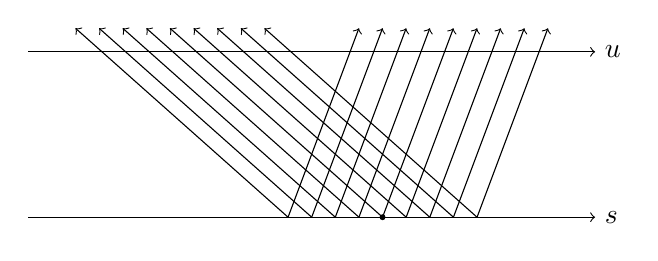
\begin{tikzpicture}[scale = 0.3, baseline]
	
		\draw[->] (-11, 0) -- (13, 0);
		\draw[->] (-11, 7) -- (13, 7);
		
		\node[right] at (13, 0) {$s$}; 
		\node[right] at (13, 7) {$u$}; 
		
		\draw[->] (0, 0) -- (-9, 8);
		\draw[->] (1, 0) -- (-8, 8);
		\draw[->] (2, 0) -- (-7, 8);
		\draw[->] (3, 0) -- (-6, 8);
		\draw[->] (4, 0) -- (-5, 8);
		\draw[->] (5, 0) -- (-4, 8);
		\draw[->] (6, 0) -- (-3, 8);
		\draw[->] (7, 0) -- (-2, 8);
		\draw[->] (8, 0) -- (-1, 8);
		
		\draw[->] (0, 0) -- (3, 8);
		\draw[->] (1, 0) -- (4, 8);
		\draw[->] (2, 0) -- (5, 8);
		\draw[->] (3, 0) -- (6, 8);
		\draw[->] (4, 0) -- (7, 8);
		\draw[->] (5, 0) -- (8, 8);
		\draw[->] (6, 0) -- (9, 8);
		\draw[->] (7, 0) -- (10, 8);
		\draw[->] (8, 0) -- (11, 8);
		
		\draw[fill] (4, 0) circle [radius = 0.1];
		
		%		\draw (0, 0) -- (0, {-sqrt(81/49 + 1)});
		%		\draw (0, 0) -- (9/7, -1);
		%		\draw (0, -1) arc (-90 : -90 + atan(9/7) : 1);
		%		
		%		\node[below right] at (0, 0) {$\theta$};
	\end{tikzpicture}

\end{document}}\hfill%
	\subcaptionbox{\label{fig:ObliqueProjectionReparameterization}}{\documentclass{standalone}
\usepackage{tikz}

\usetikzlibrary{intersections}

\begin{document}
	
	\begin{tikzpicture}[scale = 0.3, baseline]
	
		\draw[->] (-1, 0) -- (6, 0);
		\draw[name path=uAxis, ->] (-1, 7) -- (6, 7);
		
		\draw[name path=ray, ->] (0, 0) -- (5, 8);
		\node[above left] {$s$};
		
		\draw[fill] (0, 0) circle [radius = 0.1];
		\draw[fill] (0, 7) circle [radius = 0.1];
		
		\fill[name intersections={of=uAxis and ray, total=\t}]
		\foreach \s in {1,...,\t}{(intersection-\s) circle[radius = 0.1] node[below right] {$u$}};
		
		\draw (0, 0) -- (0, 3.5);
		\draw (0, 3) arc (90 : 90 - atan(5/8) : 3);
		\node at (0.55, 2) {$\theta$};
		
		\node[above] at (2, 7) {$u - s$};
		
		\draw[<->] (-2, 0) -- (-2, 7);
		\node[left] at (-2, 3.5) {$d$};
	
	\end{tikzpicture}
	
\end{document}}
	\caption[Parameterization for light fields from oblique projections]
			{(a) Light field acquisition using oblique projection. 
			 (b) Re-parameterization of the two-plane representation to angular coordinates.}
\end{figure}

\subsection*{Perspective Projection}
% Parameterization, two main types: global or relative
% Reparameterization: Orthographic <-> Perspective

Another way to capture the light field is with a grid of optical systems, e.g. cameras.
Typically, the $(u, v)$-plane is sampled on a grid $G_{uv} = \left \{ \left( u_i, v_j \right) \mid i = 1,\dots, n, j = 1, \dots, m\right \}$ on the $(u, v)$-plane with a resolution $n \times m$.
The extent in horizontal (vertical) direction is called the horizontal (vertical) \textbf{baseline}.
Although it is strictly speaking not correct, the resolution of the $(u, v)$-plane is often referred to as the angular resolution. 
The angles of the rays in a light field captured by perspective projections are determined by the focal length, the sensor size and the sensor resolution of the camera.
For a camera light field, typically it is expected that
\begin{itemize}
	\item All cameras are placed at grid positions in $G_{uv}$ on the same plane, called the $(u, v)$-plane, 
	\item The optical axes of the cameras are orthogonal to the $(u, v)$-plane, 
	\item All cameras have the same intrinsic parameters (e.g. focal length).
\end{itemize}
In this case, the focal planes of all cameras coincide with a common focal plane, the $(s, t)$-plane.
Figure~\ref{fig:ShiftedPerspectiveProjection} shows this scenario for three cameras in two dimensions.
Given images $I_{uv}(x, y)$ with respect to a coordinate system centered at the camera position $(u, v)$, the coordinates on the $(s, t)$-plane are $s = u + x$, and $t = v + y$.
Thus, the light field in continuous coordinates is obtained by 
\begin{equation}
	L(u, v, s, t) = L(u, v, u + x, v + y) = I_{uv}(x, y).
\end{equation}
In the discrete case, each camera captures sample points on the $(s, t)$-plane, but not everyone of these sample points on the $(s, t)$-plane is captured by every camera.
So, as demonstrated in figure~\ref*{fig:RectifiedPerspectiveProjection}, the camera images need to be rectified such that all discrete coordinates $(u, v, s, t)$ correspond to valid rays.
This rectification process is equivalent to a re-parameterization $L^\prime$ of the continuous light field $L$, given by the formula
\begin{equation}\label{eq:two_plane_reparameterization}
	L^\prime (u, v, s^\prime, t^\prime) = L \left(u, v, \gamma (s^\prime - u) + u, \gamma (t^\prime - v) + v \right), 
\end{equation}
where $\gamma = \frac{d}{d^\prime}$ and $d^\prime$ is the distance between the $(u, v)$-plane and the new \mbox{$(s^\prime, t^\prime)$-plane}.
As derived by \cite{DynamicallyReparameterizedLF}, this re-parameterization is equivalent to a 4D shear.

A different way to understand this coordinate change is to imagine the $(u, v)$- and $(s, t)$-plane being the aperture and sensor planes respectively, resulting in one big camera in which a light field is formed.
Changing the distance between the two planes is now equivalent to changing the focal length of this one camera.
The effect on the light field inside is similar to refocusing, except that in a conventional camera, the image on the sensor is formed by a weighted integral over $u$ and $v$ such that the angular information vanishes.
Objects at focal distance from the camera would appear sharp and objects away from the focal point would become blurred.
\todo{Refer to section about the plenoptic camera}

From stereo vision, it is known that the displacement of the projections in the image planes of two cameras is only dependent on the focal length $f$, the baseline $\Delta u$ and the distance $z$, and the relation is given by $\Delta x = f \Delta u / z$.
This knowledge can directly be applied to the two-plane parameterization. 
For the continuous light field, it amounts to
\begin{equation}\label{eq:disparity_for_two_plane_parameterization}
	\textrm{d}s = \frac{z - Z_{st}}{z - Z_{uv}} \, \textrm{d}u 
	\qquad
	\text{and} 
	\qquad
	\textrm{d}t = \frac{z - Z_{st}}{z - Z_{uv}} \, \textrm{d}v,
\end{equation}
with $Z_{uv}$ and $Z_{st}$ denoting the placement of the $(u, v)$- and \mbox{$(s, t)$-planes} in \mbox{$Z$-direction}.
Usually, the coordinate system is chosen such that $Z_{uv} = 0$.
In the discrete case, the displacement $\Delta s$ or $\Delta t$ is also called the \textbf{disparity} and is often measured in pixel units.

\begin{figure}[tb]
	\subcaptionbox{\label{fig:ShiftedPerspectiveProjection}}{\documentclass{standalone}
\usepackage{tikz}

\begin{document}
	
	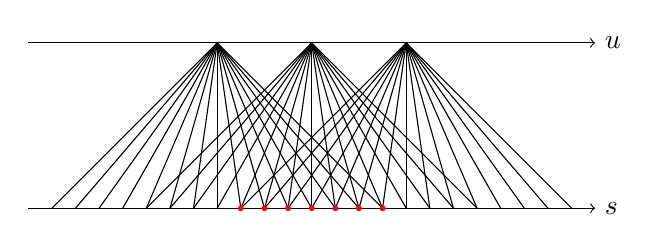
\begin{tikzpicture}[scale = 0.3]
		
		\draw[->] (-9, 0) -- (15, 0);
		\draw[->] (-9, 7) -- (15, 7);
		
		\node[right] at (15, 0) {$s$};
		\node[right] at (15, 7) {$u$};
		
		\draw (-1, 7) -- (-8, 0);
		\draw (-1, 7) -- (-7, 0);
		\draw (-1, 7) -- (-6, 0);
		\draw (-1, 7) -- (-5, 0);
		\draw (-1, 7) -- (-4, 0);
		\draw (-1, 7) -- (-3, 0);
		\draw (-1, 7) -- (-2, 0);
		\draw (-1, 7) -- (-1, 0);
		\draw (-1, 7) -- (0, 0);
		\draw (-1, 7) -- (1, 0);
		\draw (-1, 7) -- (2, 0);
		\draw (-1, 7) -- (3, 0);
		\draw (-1, 7) -- (4, 0);
		\draw (-1, 7) -- (5, 0);
		\draw (-1, 7) -- (6, 0);
		
		\draw (3, 7) -- (-4, 0);
		\draw (3, 7) -- (-3, 0);
		\draw (3, 7) -- (-2, 0);
		\draw (3, 7) -- (-1, 0);
		\draw (3, 7) -- (0, 0);
		\draw (3, 7) -- (1, 0);
		\draw (3, 7) -- (2, 0);
		\draw (3, 7) -- (3, 0);
		\draw (3, 7) -- (4, 0);
		\draw (3, 7) -- (5, 0);
		\draw (3, 7) -- (6, 0);
		\draw (3, 7) -- (7, 0);
		\draw (3, 7) -- (8, 0);
		\draw (3, 7) -- (9, 0);
		\draw (3, 7) -- (10, 0);
		
		\draw (7, 7) -- (0, 0);
		\draw (7, 7) -- (1, 0);
		\draw (7, 7) -- (2, 0);
		\draw (7, 7) -- (3, 0);
		\draw (7, 7) -- (4, 0);
		\draw (7, 7) -- (5, 0);
		\draw (7, 7) -- (6, 0);
		\draw (7, 7) -- (7, 0);
		\draw (7, 7) -- (8, 0);
		\draw (7, 7) -- (9, 0);
		\draw (7, 7) -- (10, 0);
		\draw (7, 7) -- (11, 0);
		\draw (7, 7) -- (12, 0);
		\draw (7, 7) -- (13, 0);
		\draw (7, 7) -- (14, 0);
		
		\draw[fill, red] (0, 0) circle [radius = 0.1];
		\draw[fill, red] (1, 0) circle [radius = 0.1];
		\draw[fill, red] (2, 0) circle [radius = 0.1];
		\draw[fill, red] (3, 0) circle [radius = 0.1];
		\draw[fill, red] (4, 0) circle [radius = 0.1];
		\draw[fill, red] (5, 0) circle [radius = 0.1];
		\draw[fill, red] (6, 0) circle [radius = 0.1];
	\end{tikzpicture}
	
\end{document}}\hfill%
	\subcaptionbox{\label{fig:RectifiedPerspectiveProjection}}{\documentclass{standalone}
\usepackage{tikz}

\begin{document}
	
	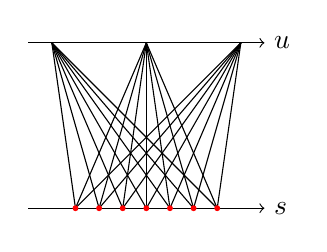
\begin{tikzpicture}[scale = 0.3]
		
		\draw[->] (-2, 0) -- (8, 0);
		\draw[->] (-2, 7) -- (8, 7);
		
		\node[right] at (8, 0) {$s$};
		\node[right] at (8, 7) {$u$};
		
		\draw (-1, 7) -- (0, 0);
		\draw (-1, 7) -- (1, 0);
		\draw (-1, 7) -- (2, 0);
		\draw (-1, 7) -- (3, 0);
		\draw (-1, 7) -- (4, 0);
		\draw (-1, 7) -- (5, 0);
		\draw (-1, 7) -- (6, 0);
		
		\draw (3, 7) -- (0, 0);
		\draw (3, 7) -- (1, 0);
		\draw (3, 7) -- (2, 0);
		\draw (3, 7) -- (3, 0);
		\draw (3, 7) -- (4, 0);
		\draw (3, 7) -- (5, 0);
		\draw (3, 7) -- (6, 0);
		
		\draw (7, 7) -- (0, 0);
		\draw (7, 7) -- (1, 0);
		\draw (7, 7) -- (2, 0);
		\draw (7, 7) -- (3, 0);
		\draw (7, 7) -- (4, 0);
		\draw (7, 7) -- (5, 0);
		\draw (7, 7) -- (6, 0);
		
		\draw[fill, red] (0, 0) circle [radius = 0.1];
		\draw[fill, red] (1, 0) circle [radius = 0.1];
		\draw[fill, red] (2, 0) circle [radius = 0.1];
		\draw[fill, red] (3, 0) circle [radius = 0.1];
		\draw[fill, red] (4, 0) circle [radius = 0.1];
		\draw[fill, red] (5, 0) circle [radius = 0.1];
		\draw[fill, red] (6, 0) circle [radius = 0.1];
		
	\end{tikzpicture}
	
\end{document}}
	\caption[Parameterization for light fields from perspective projections]
			{Perspective projections of a scene. 
			 (a) Projections with three pinhole cameras. 
			 (b) Discarding unused rays corresponds to cropping the camera images.}
\end{figure}

\section{Visualization}
\label{sec:Visualization}
\todo{Mention other types of visualization? 2D grid of images, etc.}
The epipolar-plane image (EPI) allows for a very intuitive visualization of depth from a 4D light field.
It was first defined by~\cite{EPI} as follows.
Consider a point $P$ in 3D space and a pair of cameras with the optical axis pointing in the same direcion.
The plane passing through $P$ and the two centers of projection is called the \textbf{epipolar plane}.
The epipolar plane projects to a line on each of the camera image planes, named the \textbf{epipolar line}.
This line represents a constraint for the projection of $P$ in each of the images and it is used to solve the correspondance problem in computer vision.
The notion of epipolar lines can be directly applied to a multiple camera setup.
In figure~\ref{fig:epi_example_perspective}, a synthetic scene is rendered in 500 different positions along a horizontal baseline.
Since the camera movement is in horizontal direction only, the epipolar lines correspond to a fixed pixel row in each image.
The EPIs shown in figures~\ref{fig:epi_1x500x1000x1000_scanline1} and ~\ref{fig:epi_1x500x1000x1000_scanline2} are created by collecting the chosen pixel row (scanline) in every image and stacking it up.

As described in the previous section, the depth component of $P$ occurs as a displacement of the projections in consecutive images.
Under the assumption that the $(u, v)$-plane is sampled uniformly, the disparity $D$ with respect to $P$ stays constant from one image to the next.
Thus, following the projection of the point $P$ in every image corresponds to a line in the EPI with a slope proportional to $1 / D$.
\cite{EPI} refer to this line as the \textbf{feature path}.
This means that points farther away from the camera will appear as a feature path in the EPI with steeper slope than points close to the camera.
Note that the depth range in the light field can immediately be determined by identifying the maximum and minimum slope in the EPI.
Also, for a perfectly Lambertian scene, each line in the EPI has a uniform color.

\begin{figure}[tb]
	\subcaptionbox{\label{fig:epi_1x500x1000x1000_overview}}{\documentclass{standalone}
\usepackage{tikz}
\usepackage{pgfplots}

\begin{document}
	\begin{tikzpicture}[baseline]
		\begin{axis}[	scale only axis,
						height = 2.8cm,
						ylabel near ticks,
						xlabel near ticks, 
						ticks = none, 
						enlargelimits = true, 
						axis on top, 
						axis equal image,
						axis lines = left,
						xlabel = {$x$},
						ylabel = {$y$} 
					]
	
			\addplot graphics [xmin = 0, xmax = 1000, ymin = 0, ymax = 615] {epi_1x500x1000x1000/overview};
		
			\addplot[mark = none, red] coordinates {(0, 615 - 497) (1000, 615 - 497)};
			\addplot[mark = none, red] coordinates {(0, 615 - 236) (1000, 615 - 236)};
			
		\end{axis}
	\end{tikzpicture}	
\end{document}
}\hfill%
	\subcaptionbox{\label{fig:epi_1x500x1000x1000_scanline1}}{\documentclass{standalone}
\usepackage{tikz}
\usepackage{pgfplots}

\begin{document}
	\begin{tikzpicture}[baseline]
		\begin{axis}[	scale only axis,
						height = 2.8cm,
						xtick = {0, 1000}, 
						ytick = {0, 500},
						ylabel near ticks,
						xlabel near ticks, 
						ticks = none, 
						enlargelimits = true, 
						axis on top, 
						axis equal image,
						axis lines = left, 
						xlabel = {$x$}, 
						ylabel = {$u$}
					]
	
			\addplot[plot graphics/node/.append style={yscale=-1,anchor=north west}] % Flip EPI vertically (MATLAB matrix)
					graphics [xmin = 0, xmax = 1000, ymin = 0, ymax = 500] {epi_1x500x1000x1000/scanY=379};
		
		\end{axis}
	\end{tikzpicture}	
\end{document}

}\hfill%
	\subcaptionbox{\label{fig:epi_1x500x1000x1000_scanline2}}{\documentclass{standalone}
\usepackage{tikz}
\usepackage{pgfplots}

\begin{document}
	\begin{tikzpicture}[baseline]
		\begin{axis}[	scale only axis,
						height = 2.8cm,
						xtick = {0, 1000}, 
						ytick = {0, 500},
						ylabel near ticks,
						xlabel near ticks, 
						ticks = none, 
						enlargelimits = true, 
						axis on top, 
						axis equal image,
						axis lines = left, 
						xlabel = {$x$}, 
						ylabel = {$u$}
					]
	
			\addplot[plot graphics/node/.append style={yscale=-1,anchor=north west}] % Flip EPI vertically (MATLAB matrix)
					graphics [xmin = 0, xmax = 1000, ymin = 0, ymax = 500] {epi_1x500x1000x1000/scanY=641};
			
		\end{axis}
	\end{tikzpicture}	
\end{document}}
	\\
	\subcaptionbox{\label{fig:epi_1x500x1000x1000_overview_rectified}}{\documentclass{standalone}
\usepackage{tikz}
\usepackage{pgfplots}

\begin{document}
	\begin{tikzpicture}[baseline]
		\begin{axis}[	scale only axis,
						height = 3.2cm,
						ylabel near ticks,
						xlabel near ticks, 
						ticks = none, 
						enlargelimits = true, 
						axis on top, 
						axis equal image,
						axis lines = left,
						xlabel = {$x$},
						ylabel = {$y$} 
					]
	
			\addplot graphics [xmin = 125, xmax = 875, ymin = 0, ymax = 615] {figures/epi_1x500x1000x1000/rectified/overview};
		
			\addplot[mark = none, black] coordinates {(0, 615 - 497) (1000, 615 - 497)};
			\addplot[mark = none, black] coordinates {(0, 615 - 236) (1000, 615 - 236)};
			
			\only<2>{\addplot[mark = none, red] coordinates {(0, 615 - 497) (1000, 615 - 497)};}
			\only<1>{\addplot[mark = none, red] coordinates {(0, 615 - 236) (1000, 615 - 236)};}
			
		\end{axis}
	\end{tikzpicture}	
\end{document}}\hfill%
	\subcaptionbox{\label{fig:epi_1x500x1000x1000_scanline1_rectified}}{\documentclass{standalone}
\usepackage{tikz}
\usepackage{pgfplots}

\begin{document}
	\begin{tikzpicture}[baseline]
		\begin{axis}[	scale only axis,
						height = 2.8cm,
						xtick = {0, 1000}, 
						ytick = {0, 500},
						ylabel near ticks,
						xlabel near ticks, 
						ticks = none, 
						enlargelimits = true, 
						axis on top, 
						axis equal image,
						axis lines = left, 
						xlabel = {$x$}, 
						ylabel = {$u$}
					]
	
			% Add dummy line to set the size of the coordinate system
			\addplot[mark = none, white] coordinates {(0, 0) (1000, 0)};
	
			\addplot[plot graphics/node/.append style={yscale=-1,anchor=north west}] % Flip EPI vertically (MATLAB matrix)
					graphics [xmin = 125, xmax = 875, ymin = 0, ymax = 500] {epi_1x500x1000x1000/rectified/scanY=379};
		
		\end{axis}
	\end{tikzpicture}	
\end{document}}\hfill%
	\subcaptionbox{\label{fig:epi_1x500x1000x1000_scanline2_rectified}}{\documentclass{standalone}
\usepackage{tikz}
\usepackage{pgfplots}

\begin{document}
	\begin{tikzpicture}[baseline]
		\begin{axis}[	scale only axis,
						height = 3.2cm,
						xtick = {0, 1000}, 
						ytick = {0, 500},
						ylabel near ticks,
						xlabel near ticks, 
						ticks = none, 
						enlargelimits = true, 
						axis on top, 
						axis equal image,
						axis lines = left, 
						xlabel = {$x$}, 
						ylabel = {$u$}
					]
	
			% Add dummy line to set the size of the coordinate system
			\addplot[mark = none, white] coordinates {(0, 0) (1000, 0)};
	
			\addplot[plot graphics/node/.append style={yscale=-1,anchor=north west}] % Flip EPI vertically (MATLAB matrix)
					graphics [xmin = 125, xmax = 875, ymin = 0, ymax = 500] {figures/epi_1x500x1000x1000/rectified/scanY=641};
			
		\end{axis}
	\end{tikzpicture}	
\end{document}}\hfill%
	\caption[Visualization of the light field with epipolar plane images]
			{(a) Raw 3D light field rendered from 500 positions along a horizontal baseline.
				 Two scanlines are extracted from every image. 
			 (b) The feature paths of the blue and green dice have a steeper slope than those of the red die.
			 (c) Feature paths of the yellow die have an even steeper slope, indicating greater depth.
			 (d) The light field is rectified according to figure~\ref{fig:RectifiedPerspectiveProjection} such that the disparities of the red die are approximately zero.
			 (e) - (f) EPIs from the same scanlines. The slopes of the feature paths stay the same relative to each other. }
	\label{fig:epi_example_perspective}
\end{figure}

\section{The Plenoptic Camera}

\todo{Introduce Lytro Camera, mention refocusing}
\todo{Produce figure showing the "aperture view" with the circular drop-off.}
\todo{Produce figure showing the "lenslet" view}